
\chapter{Sprint 3}
\label{Sprint3}
\lhead{Chapter 9. \emph{Sprint 3}}

\section{Duration}
The duration of the sprint was the following:
\begin{itemize}
\item Sprint start:  October, 7th
\item Milestone M2 (mid-term report delivery): October, 14th.
\item Sprint end: October, 20th
\end{itemize}

\section{Planning}

The last sprint had proceeded without issues, so we didn't make any big adjustments to our plan for this iteration. 
We planned to focus on report work and do some more development after achieving milestone M2.

We understood that mid-term delivery was a good chance to receive valuable feedback from the student advisor, the technical advisor and the customer so we directed most of our efforts in report writing in order to receive as much feedback as possible on it.

We prepared a separate work plan for our colleague in Oslo with a focus on documentation
writing since we thought it would be easier for him and for us to work collaboratively
on the report rather than development.

\iffalse
The first week the whole team would focus on writing the report
%The plan consisted on report writing for the first week,
in order to receive as much feedback as possibile on it. 
%This task was assigned to the whole team.
For the second week, %in view of our customer's visit to Trondheim on the last days of the month,
we planned to proceed with system and application development %after mid-term delivery
in order to implement most of the functionality for the second product prototype meanwhile
our colleague in Oslo would continue to write the report.
%as well as some additional work on the report to be done by our colleague in Oslo.

%assigning him some work on the report for the second week of the sprint as well.
\fi

\section{Goal(s)}

The goal of this sprint was the mid-term delivery of the report; this corresponded to
the second project's milestone M2. Furthermore, another goal was finalizing the design and continuing
the development of the second prototype of the product.% which would feature HealthVault interoperability.


\section{Results and feedback}

We were able to write what we planned to in the report and had no problem meeting the deadline for the midterm delivery. 
We were generally satisfied with the quality of what had been written having spent some time reviewing the document to ensure consistency and a logical flow.
We attended the lecture about technical writing and at the end of which we received some positive feedback on the report.

Development proceeded without major issues. 
We were able to re-use good portions of code provided by HealthVault's SDK, dramatically reducing the time spent on development.
We performed some major refactoring of the code on a dedicated Git branch in an effort to a achieve a more \'neat\' deployment solution which didn't require a separate servlet container like Apache Tomcat but was entirely based on Spring, using an embedded servlet-container.

During one of the meetings with the customer, we scheduled a demonstration of the product for the 24th of October when he would travel to Trondheim for work.

\section{Evaluation}

\begin{figure}
\centering
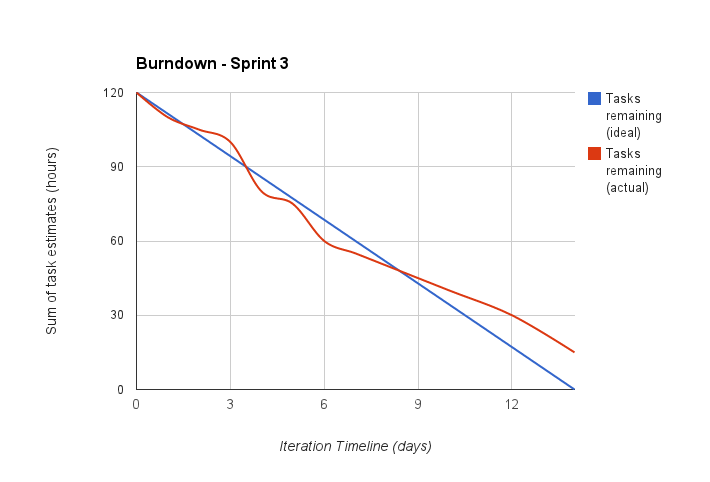
\includegraphics[scale=0.60]{../Figures/burndownSprint3.png}
\caption{Iteration burndown chart}
\label{figure:burndownsprint3}
\end{figure}

All in all this sprint was successful because we managed to meet the deadline for report delivery.
Additionally, we were glad to have received positive feedback on our report.

However, refactoring was an unexpectedly time-consuming task and did not achieve expected results.
Luckily, since all refactoring had been performed on a separte branch on Git, it didn't create problems as we always had a working branch for development and demonstration purposes.

By the end of the sprint it became clear that the customer wasn't that interested in a prototype application for Withings. 
However, because one team member owned a Withings scale device, we thought it would have been a good idea to include that in the demonstration.
Since Withings supported integration with HealthVault natively, we came up with the following scenario for product demonstration:
\begin{enumerate}[1)]
\item the user steps on the scale
\item the weight is acquired by the scale and sent to Withings
\item the measurement on Withings is automatically integrated in HealthVault
\item the Android application fetches the measurement from HealthVault
\item the measurement is sent to our integration platform
\end{enumerate}
Regarding our collaboration with our colleague in Oslo, he didn't report the time he spent on the project correctly, and his contribution was discontinuos because he had begun to work full-time.
This didn't create any big problems because development had proceeded smoothly so other team members had some spare time to cover up for that.
This iteration burndown chart is shown in figure \ref{figure:burndownsprint3}.

\clearpage
\section{Backlog}
See below the sprint backlog.

\begin{enumerate}[1.]
\item \textbf{M2 Mid-term report}:
	delivery of the mid-term report
\item \textbf{Project management} included:
	\begin{itemize}
		\item \textbf{Sprint startup meeting}:
			included sprint planning and review
		\item \textbf{Weekly meetings}: 
			with both the customer and the supervisor. Internal meeting with our colleague in Oslo
		\item \textbf{Meeting notes}:
			taking notes during meetings, reviewing of the notes
		\item \textbf{Status reports}:
			for both week 41 and 42
		\item \textbf{Risk analysis}:
			updated on a weekly basis
	\end{itemize}
	\item \textbf{Weighter Application development}\newline
		continued development of the Android application
	\item \textbf{System development}\newline
		study different ways to deploy the backend
		1) as a WAR file in a separate servlet container (Apache Tomcat) or 2) as a Spring JAR file
		with embedded servlet support. Furthermore we continued development
	\item \textbf{Report work}\newline
		to be done by the team member in Trondheim
	\item \textbf{Additional report work}\newline
		to be done by the team member in Oslo
	\item \textbf{Testing}\newline
		perform unit testing
\end{enumerate}
